\documentclass[11pt]{article}
    \title{\textbf{Topology optimization applied to hydrogeological problems}}
    \author{Moise Rousseau, Thomas Pabst}
    \date{}
    
    \addtolength{\topmargin}{-3cm}
    \addtolength{\textheight}{3cm}
    
\usepackage{amsmath}
\usepackage{amssymb}
\usepackage{graphicx}

\begin{document}


\maketitle
\thispagestyle{empty}

\section*{Abstract}



\section{Introduction}

Optimisation in Geoscience (example and other)

Minimize a function could be hard if the function is complex. Numerous method: gradient descent and derivative free (genetic algo, black box method and other, stochastic).
Traditional method for minimize a function is to use gradient descent
Minimise could be done using requires the gradient of 

Optimization with high number of variable in geophysics, use adjoint method

Other use of adjoint method in other field: topology optimization 

Thus, possible to use to optimize 2 materials distribution

While forward sensitivity analysis is best suited to the situation of finding the sensitivities of a potentially large number of solution variables with respect to a small number of parameters, reverse (adjoint) sensitivity analysis is best suited to the complementary situation of finding the sensitivity of a scalar (or small-dimensional) function of the solution with respect to a large number of parameter (Cao et al. 2003).

Some problems require the sensitivities with respect to a large number of parameters. For these problems, particularly if the number of state variables is also large, the forward sensitivity approach is intractable. These problems can often be handled more efficiently by the adjoint method (Errico 1997). From (Cao et al. 2003)




\section{Methodology}

\subsection{Overview}

Topology optimization for finite volume method: 



\subsection{Sensitivity analysis using adjoint method}

Let $X_i(p)$ ($1 \leq i \leq n$) be the properties of a discretized domain (such as permeability, porosity, or dispersivity for example) continuously parametrized with $p$ the continuous parameter.
Let $P$ be the pressure solution to the discretized Richards flow equation and $C$ the concentration solution to the discretized advective-dispersive reactive transport equation. Both solution $P$ and $C$ depend on the discretized material properties $X_i(p)$.
The solving process of the discretized Richard's equation and of the reactive transport equation generally consist of finding the root of the iscretized linear system of equation residual. Therefore, the pressure $P$ and concentration $C$ and given by $R_P(X_i, P)=0$ and $R_C(X_i, P, C)=0$ with $\partial R_P / \partial P$ and $\partial R_C / \partial C$ everywhere non-singular.
The objective of sensitivity analysis is to find the total derivative of the real-valued cost function noted $c$ according to the material distribution $dc\left(X_i, P, C\right) / dp$.

Total derivative of the cost function $c$ could be expanded using the chain rules:
\begin{equation}
\frac{dc}{dp} = 
\frac{\partial c}{\partial P}\frac{\partial P}{\partial p} + 
\frac{\partial c}{\partial C}\frac{\partial C}{\partial p} + 
\sum_{i=1}^n \frac{\partial c}{\partial X_i}\frac{\partial X_i}{\partial p}
\end{equation}
In the above, the terms $\frac{\partial c}{\partial P}$, $\frac{\partial c}{\partial C}$, $\frac{\partial c}{\partial X_i}$ and $\frac{\partial X_i}{\partial p}$ are easy to compute. However, the other terms $\frac{\partial P}{\partial p}$ and $\frac{\partial C}{\partial p}$ representing the derivative of the pressure and concentration solutions according to the material parameter $p$ is non-trivial to obtain. Expanding the derivative of the residual function $R_P$ and $R_C$ leads:
\begin{subequations}
\begin{align}
\frac{dR_P}{dp} =
\frac{\partial R_P}{\partial P}\frac{\partial P}{\partial p} +
\sum_{i=1}^n \frac{\partial R_P}{\partial X_i}\frac{\partial X_i}{\partial p} = 0
\\
\frac{dR_C}{dp} = 
\frac{\partial R_C}{\partial P}\frac{\partial P}{\partial p} +
\frac{\partial R_C}{\partial C}\frac{\partial C}{\partial p} +
\sum_{i=1}^n \frac{\partial R_C}{\partial X_i}\frac{\partial X_i}{\partial p} = 0
\end{align}
\end{subequations}
The previous expression could be rewrite using block matrix product to express the derivative of the pressure $P$ and concentration $C$ according to the parameter $p$:
\begin{equation}
\begin{pmatrix}
\frac{\partial P}{\partial p} \\ \frac{\partial C}{\partial p}
\end{pmatrix}
= -
\begin{pmatrix}
\frac{\partial R_P}{\partial P} & 0 \\ 
\frac{\partial R_C}{\partial P} & \frac{\partial R_C}{\partial C}
\end{pmatrix}^{-1} \cdot
\ \sum_{i=1}^n 
\begin{pmatrix}
\frac{\partial R_P}{\partial X_i}\frac{\partial X_i}{\partial p} \\ \frac{\partial R_C}{\partial X_i}\frac{\partial X_i}{\partial p}
\end{pmatrix}
\end{equation}
Then, the total derivative of the cost function could also be write with matrix block:
\begin{equation}
\frac{dc}{dp}
=
\begin{pmatrix}
\frac{\partial c}{\partial P}^T & \frac{\partial c}{\partial C}^T
\end{pmatrix} \cdot
\begin{pmatrix}
\frac{\partial P}{\partial p} \\ \frac{\partial C}{\partial p}
\end{pmatrix} \ + \ 
\sum_{i=1}^n \frac{\partial c}{\partial X_i}\frac{\partial X_i}{\partial p}
\end{equation}
Which leads:
\begin{equation}
\frac{dc}{dp}
= -
\begin{pmatrix}
\frac{\partial c}{\partial P}^T & \frac{\partial c}{\partial C}^T
\end{pmatrix}
\begin{pmatrix}
\frac{\partial R_P}{\partial P} & 0 \\ 
\frac{\partial R_C}{\partial P} & \frac{\partial R_C}{\partial C}
\end{pmatrix}^{-1} \sum_{i=1}^n 
\begin{pmatrix}
\frac{\partial R_P}{\partial X_i}\frac{\partial X_i}{\partial p} \\ \frac{\partial R_C}{\partial X_i}\frac{\partial X_i}{\partial p}
\end{pmatrix}+
\sum_{i=1}^n \frac{\partial c}{\partial X_i}\frac{\partial X_i}{\partial p}
\end{equation}
The first matrix multiplication between the cost function derivative and the pressure and the inverse residual derivative could be interpreted as a matrix-vector product which is easy to solve numerically such as:
\begin{equation}
\begin{pmatrix}
\frac{\partial R_P}{\partial P}^T & \frac{\partial R_C}{\partial P}^T \\ 
0 & \frac{\partial R_C}{\partial C}^T
\end{pmatrix} \cdot \lambda^T
= 
\begin{pmatrix}
\frac{\partial c}{\partial P} \\ \frac{\partial c}{\partial C}
\end{pmatrix}
\end{equation}
Therefore, the total derivative of the cost function writes:
\begin{equation}
\frac{dc}{dp}
= -
\lambda \cdot \sum_{i=1}^n 
\begin{pmatrix}
\frac{\partial R_P}{\partial X_i}\frac{\partial X_i}{\partial p} \\ \frac{\partial R_C}{\partial X_i}\frac{\partial X_i}{\partial p}
\end{pmatrix}+
\sum_{i=1}^n \frac{\partial c}{\partial X_i}\frac{\partial X_i}{\partial p}
\end{equation}




\subsection{Implementation}

"Rather than on in-house codes, the car industry relies almost exclusively on commercial CFD software." obstacle for implementing adjoint method. %https://mathematicsinindustry.springeropen.com/articles/10.1186/2190-5983-4-6

The proposed method was implemented into the open-source finite volume code PFLOTRAN. PFLOTRAN solves the 

\begin{figure}[]
  \centering
  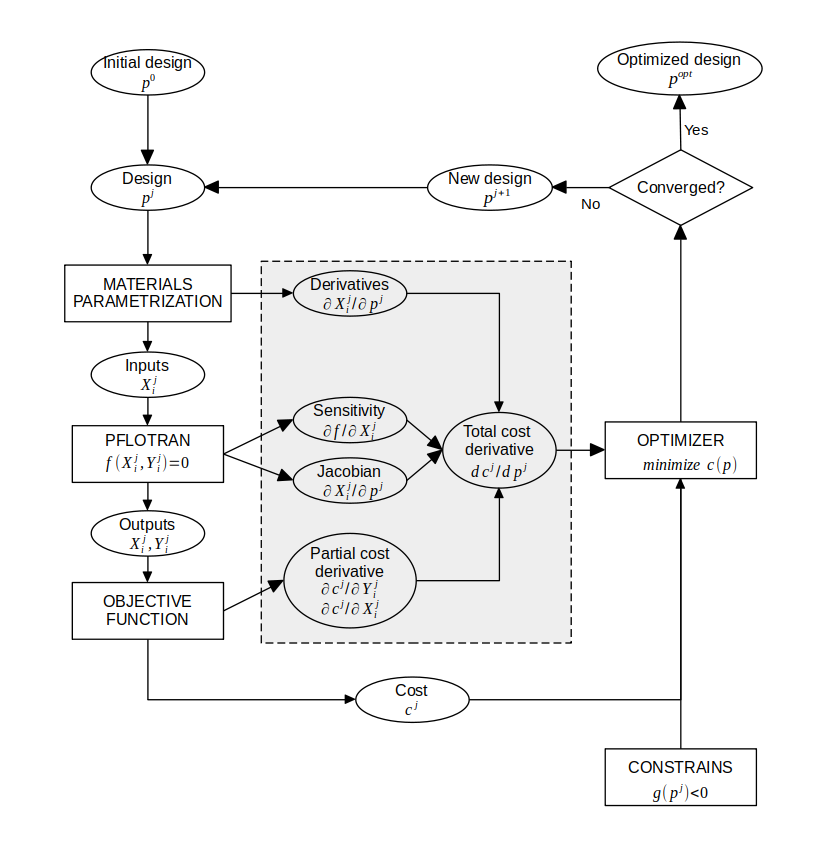
\includegraphics[width=\textwidth]{figures/implementation_scheme.png}
  \label{cases_figure}
  \caption{Remplacer PFLOTRAN par SOLVER. Jacobian and Sensitivity inversé... Schematics of a possible implementation of the topology optimization method for an existing solver.}
\end{figure}

Sensitivity are computed using finite difference method, which allow to reuse FORTRAN subroutine computing the derivatives of the residual.




\section{Application}

Transmissivity field estimation: https://agupubs.onlinelibrary.wiley.com/doi/full/10.1029/2008WR007033

Optimization of drain location

Pumping well for dewatering

Minimisation of fresh groundwater fluxes inside reactive waste

Optimal placement of reactive barrier

Reduction of transient oxydation of mine waste



\section{Discussion}
-
Comparison of continuous adjoint and finite difference adjoint %https://arc.aiaa.org/doi/pdf/10.2514/6.2000-667


\section{Conclusion}



\end{document}

